%%%%%%%%%%%%%%%%%%%%%%%%%%%%%%%%%%%%%%%%%
% Journal Article
% LaTeX Template
% Version 1.4 (15/5/16)
%
% This template has been downloaded from:
% http://www.LaTeXTemplates.com
%
% Original author:
% Frits Wenneker (http://www.howtotex.com) with extensive modifications by
% Vel (vel@LaTeXTemplates.com)
%
% License:
% CC BY-NC-SA 3.0 (http://creativecommons.org/licenses/by-nc-sa/3.0/)
%
%%%%%%%%%%%%%%%%%%%%%%%%%%%%%%%%%%%%%%%%%

%----------------------------------------------------------------------------------------
%	PACKAGES AND OTHER DOCUMENT CONFIGURATIONS
%----------------------------------------------------------------------------------------

\documentclass[twoside,twocolumn]{article}

\usepackage{blindtext} % Package to generate dummy text throughout this template 

\usepackage[sc]{mathpazo} % Use the Palatino font
\usepackage[T1]{fontenc} % Use 8-bit encoding that has 256 glyphs
\linespread{1.05} % Line spacing - Palatino needs more space between lines
\usepackage{microtype} % Slightly tweak font spacing for aesthetics

\usepackage[english]{babel} % Language hyphenation and typographical rules

\usepackage[hmarginratio=1:1,top=32mm,columnsep=20pt,a4paper,total={6in,9in}]{geometry} % Document margins
\usepackage[hang, small,labelfont=bf,up,textfont=it,up]{caption} % Custom captions under/above floats in tables or figures
\usepackage{booktabs} % Horizontal rules in tables

\usepackage{lettrine} % The lettrine is the first enlarged letter at the beginning of the text

\usepackage{enumitem} % Customized lists
\setlist[itemize]{noitemsep} % Make itemize lists more compact

\usepackage{abstract} % Allows abstract customization
\renewcommand{\abstractnamefont}{\normalfont\bfseries} % Set the "Abstract" text to bold
\renewcommand{\abstracttextfont}{\normalfont\small\itshape} % Set the abstract itself to small italic text

\usepackage{titlesec} % Allows customization of titles
\renewcommand\thesection{\Roman{section}} % Roman numerals for the sections
\renewcommand\thesubsection{\roman{subsection}} % roman numerals for subsections
\titleformat{\section}[block]{\large\scshape\centering}{\thesection.}{1em}{} % Change the look of the section titles
\titleformat{\subsection}[block]{\large}{\thesubsection.}{1em}{} % Change the look of the section titles

\usepackage{fancyhdr} % Headers and footers
\pagestyle{fancy} % All pages have headers and footers
\fancyhead{} % Blank out the default header
\fancyfoot{} % Blank out the default footer
\fancyhead[C]{Game of Life  $\bullet$ Computer Systems A $\bullet$ December 2022} % Custom header text
\fancyfoot[RO,LE]{\thepage} % Custom footer text

\usepackage{titling} % Customizing the title section

\usepackage{hyperref} % For hyperlinks in the PDF
\usepackage{graphicx}
\graphicspath{{./img/}}
\usepackage{algorithm}
\usepackage{algpseudocode}
\usepackage{txfonts}

%----------------------------------------------------------------------------------------
%	TITLE SECTION
%----------------------------------------------------------------------------------------

\setlength{\droptitle}{-4\baselineskip} % Move the title up

\pretitle{\begin{center}\Huge\bfseries} % Article title formatting
\posttitle{\end{center}} % Article title closing formatting
\title{A parallelised and distributed approach to implementing Conway's Game of Life} % Article title
\author{%
\textsc{Aaron Chan}\\[1ex] % Your name
\normalsize University of Bristol \\ % Your institution
\normalsize {ho21739@bristol.ac.uk} % Your email address
\and % Uncomment if 2 authors are required, duplicate these 4 lines if more
\textsc{Ferdinand Hubbard}\\[1ex] % Second author's name
\normalsize University of Bristol \\ % Your institution
\normalsize {ej21378@bristol.ac.uk} % Your email address
}
\date{\today} % Leave empty to omit a date
\renewcommand{\maketitlehookd}{
\begin{abstract}
  We intend to explain our two solutions for implementing Conway's Game of Life in Golang, namely the Parallel and Distributed versions.
  Within this report, we will discuss the impacts of thread usage in both our implementations, as well as the effect of distributed computation as opposed to single-machine computation. In essence, we found that execution time was sped up as we increased thread count, reduced branch instructions and implemented a halo exchange mechanism.
\end{abstract}
}

%----------------------------------------------------------------------------------------

\begin{document}

% Print the title
\maketitle

%----------------------------------------------------------------------------------------
%	ARTICLE CONTENTS
%----------------------------------------------------------------------------------------
\section{Introduction to the parallel solution}

As an initial attempt, we began by implementing a 
single-threaded Game of Life (GoL) Engine, expanding upon this work 
with parallelisation by virtue of concurrent go-routine workers. 
Recognising that there exists various methods to calculating the perimeter
for \texttt{getNeighbourCount}, we tried various counting methods - taking into 
account the wrap-around feature of Game of Life.

% \begin{itemize}
%   \item single threaded implementation
%   \item events passing (alive cells, turn completed)
%   \item PGM image output implementation
%   \item SDL implementation (flipped cells events)
%   \item using channels and goroutines to create multiple workers (parallelising the solution)
%   \item switching to a memory sharing solution instead of using channels (TODO?)
%   \item implementing halo exchange
% \end{itemize}
%------------------------------------------------

\section{benchmarking methodology}
Our means of evaluating parallelisation performance gains 
was via the Go testing framework. Using 512px x 512px PGM images, we 
repeated each benchmark 10 times, taking the average runtime for each thread to acquire the central value, 
and plotting them. Each feature implementation was benchmarked in the same fashion, using Linux lab machines 
with CPUs being Intel i7-8700 (6 core, 12 threads).
% \lettrine[nindent=0em,lines=3]{L} orem ipsum dolor sit amet, consectetur adipiscing elit.
% \begin{itemize}
%   \item use built in golang benchmark framework
%   \item run command ....
%   \item output to txt
%   \item run python script to plot graphs
%   \item barchart of time taken against threads used
%   \item runs benchmarks on all pgm images
%   \item repeats benchmarks until results fall within a certain standard deviation (TBC)
% \end{itemize}
%------------------------------------------------
\renewcommand\thesubsection{\Alph{subsection}}
\begin{figure}
  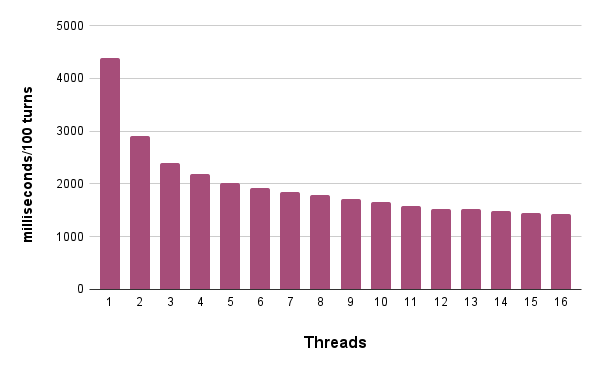
\includegraphics[width=\linewidth]{modulo.png}
  \caption{Modulo Implementation}
  \label{fig:chart1}
\end{figure}

\section{A split personality program}
\subsection{Parallelisation logic}
The baseline implementation's distributor function starts with
reading the image into 2D slice via \textit{io} commands, before evenly dividing 
the workload between workers. With the aid of go-routines, workers have access to the old slice
as well as the boundaries in which to process. By using \texttt{getNeighbourCount}, we apply the Game of Life
laws onto the world, piping results into a blank slice of size: \[( endRow - startRow ) \times ImageWidth\]
Sending the results back to the distributor, we integrate back together the new slices, move the pointer to the old world
to this newly-merged world and send the appropriate signals on the \textit{events}, \textit{io} channels.

%------------------------------------------------

\subsection{On the topic of analysis 1}

From Fig. 1, we can conclude that multithreading have an overall improvement on performance. 
There is a correlation between increasing number of threads and decreasing execution times, likely due 
to some functions, such as \texttt{getNeighbourCount}, being "embarrassingly parallelisable". We 
favour the term "delightfully parallel". As we have more cores for processing, the time taken for each turn is 
reduced, hence the curve. 

We do take notice of the obvious trend of diminishing returns - 
the gradient of the time-thread curve flattens. We attribute this to unparallelisable core tasks such as IO 
- the major slowdown that is reading and writing to/from the disk, and submit that using more threads than 
a CPU physically has causes overhead in scheduling, minimising the benefits of allocating extra threads for processing.
We suspect also that, contributing to this, the workload division does not change as much the more threads there are,
which explains the reciprocal graph shape curve.

Regarding the numerical results, we find greatest performance was with 16 threads (despite the diminishing returns)
with a 67.6\% decrease in processing time. As for the worst change in performance thread-to-thread, 
we see the 14th - 15th threads having the smallest difference in performance change (0.353\%), but acknowledge the
potential anomalous data point.

\section{How to count?}
\subsection{Counting methods}
It is well documented that division and other non-atomic arithmetic operations are slow. Thus, we submit our alternative
implementations for \texttt{getNeighbourCount}. Fig. 1, our original implementation, uses the modulo operation (\%), 
whereas Fig. 2, Fig. 3, use Branching (if-statements) and Bitmasking respectively. From this data, we see
that Bitmasking is the fastest on average, but we can identify positive notes from all three.
\subsection{On the topic of Analysis 2}
\begin{figure}
  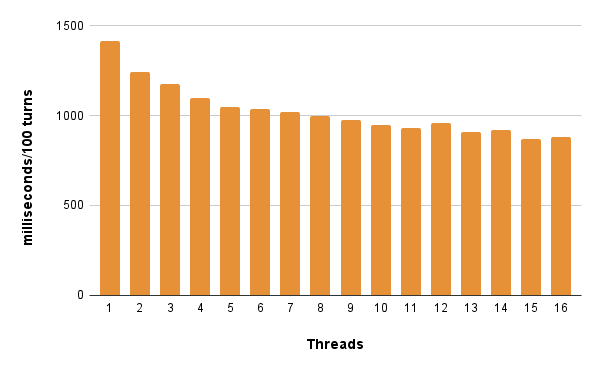
\includegraphics[width=\linewidth]{branching.png}
  \caption{Branching Implementation}
  \label{fig:chart2}
\end{figure}
\begin{figure}
  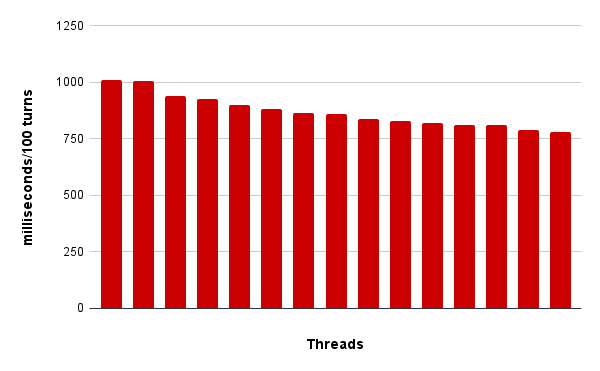
\includegraphics[width=\linewidth]{bitmask.png}
  \caption{Bitmask Implementation}
  \label{fig:chart3}
\end{figure}

Statistically-speaking, we find the solution using 
modulo operations is most affected by thread usage, having standard deviation 413ms, as opposed to 107ms 
and 73ms for branching and bitmasking respectively. Interested persons will find our results achieved by:
\[SD(\forall x \in runtimes : max(runtimes) - x)\]
As discussed before, this, however, implies not that higher threads means greater 
performance as there exists other, non-parallelisable tasks setting a base level of execution time. 
The low standard deviation of the bitmasked implementation alludes to this portion of the program being as 
near optimised as we possibly can. 

When it comes to average times for threads, bitmasking takes the lead with
890ms, followed by 1026ms and 1989ms for branching and modular respectively. This does identify branching for the 
greatest decrease in runtime, with a 74.2\% decrease, as opposed to 32.1\%.

\subsection{Our Algorithms}

Code-wise, our initial implementation for \texttt{getNeighbourCount} used modulo operators unnecessarily. It did the following:
\begin{enumerate}[noitemsep]
  \item Set row = coordinate row \% ImageHeight
  \item Set col = coordinate col \% ImageWidth
  \item If row | col < 0, then add ImageHeight/Width respectively
  \item If world[row][col] was 255, increment alive count
\end{enumerate}

With this, while it succeeds in its purpose, it does not
succeed efficiently. Areas of improvement include removal of the modulo operator, which, here,
does not serve any real purpose. This leads to our second implementation - branching:

\begin{algorithm}
  \caption{Branching getNeighbourCount}
  \begin{algorithmic}
    \State Let $i, j \gets (row, column)$ on world
  \State Let $O \gets [\{-1,0,1\} \times \{-1, 0, 1\} - \{0,0\}]$
  \State Let $alive \gets 0$   
  \For{$(x,y) \in O$}
      \State $row \gets (i + y)$
      \If{row < 0}
        \State $row \gets ImageHeight-1$
      \ElsIf{row = ImageHeight}
        \State $row \gets 0$
      \EndIf
      \State $col \gets (j + x)$
      \If{col < 0}
        \State $col \gets ImageWidth - 1$
        \ElsIf{col = ImageWidth}
          \State $col \gets 0$
      \EndIf
      \If{world[row][col] = 255}
      \State $alive++$
      \EndIf
    \EndFor
    \State \Return $alive$
  \end{algorithmic}
\end{algorithm}
Although the line count has certainly increased, the performance has drastically improved. Citing the 
74.2\% decrease, this does appear to be "good enough" as an implementation. An improvement may be to rid 
ourselves of branches, as this involves branch prediction which itself is intensive, due to how the CPU 
does not know which path will be taken ahead of time. If we use only logical operations,
we get the Bitmasking implementation:
\begin{algorithm}
  \caption{Bitmasked getNeighbourCount}
  \begin{algorithmic}
    \State Let $i, j \gets (row, column)$ on world
  \State Let $O \gets [\{-1,0,1\} \times \{-1, 0, 1\} - \{0,0\}]$
  \State Let $alive \gets 0$   
  \For{$(x,y) \in O$}
      \State $row \gets (i + y) \& (ImageHeight - 1)$
      \State $col \gets (j + x) \& (ImageWidth - 1)$
      \State $alive \gets alive + world[row][col] >> 7$
    \EndFor
    \State \Return alive
  \end{algorithmic}
\end{algorithm}

This algorithm is our fastest implementation. Minimising both line count and runtime, it 
counts the neighbours using purely bitwise operators and assignments - no branching needed.

%------------------------------------------------

\section{memory sharing}
\subsection{Motivation}
Looking at our achievements in counting, we noticed overhead associated with channel communication.
Exploring \href{https://github.com/golang/go/blob/4fc9565ffce91c4299903f7c17a275f0786734a1/src/runtime/chan.go}
{Go's implementation for channels}, we see much overhead. Since we know a channel is a thread-safe memory sharing
mechanism, we can rid the overhead, using only mutex locks and condition variables.
\subsection{Implementation}
Our homemade channel implementation does the following:
\begin{enumerate}[noitemsep]
  \item Acquire the mutex lock
  \item While \texttt{condition} is false, await broadcast unless non-blocking send
  \item Use the value, then broadcast to other processes
  \item Finally, unlock mutex
\end{enumerate}
We introduce 2 methods, \texttt{Send} \& \texttt{Receive}. \texttt{Send} waits for the memory space 
to be empty, and replaces it with a value. \texttt{Receive} waits for the memory space to point to a value, and then 
replaces it with \texttt{nil}. \texttt{Go 1.12} does not have generics, which vastly complicated implementation. 
Benchmarks with memory sharing (and bitmasked \texttt{getNeighbourCount}) is shown in Fig. 4.
\subsection{On the topic of Analysis 3}
benchmarks go here, analysis here

Lorem ipsum dolor sit amet, consectetur adipiscing elit.
\blindtext % Dummy text



%------------------------------------------------

\section{Implementing Halo Exchange}

% \lettrine[nindent=0em,lines=3]{L} orem ipsum dolor sit amet, consectetur adipiscing elit.
TO BE IMPLEMENTED
%------------------------------------------------

\section{benchmarking and critical analysis of the Halo Exchange}

\lettrine[nindent=0em,lines=3]{L} orem ipsum dolor sit amet, consectetur adipiscing elit.
TO BE IMPLEMENTED
%------------------------------------------------

\section{benchmarking and critical analysis of enabling SDL}

% \lettrine[nindent=0em,lines=3]{L} orem ipsum dolor sit amet, consectetur adipiscing elit.
\begin{itemize}
  \item show graphs and describe shape and differences of with vs without SDL
  \item explain how SDL works
  \item explain how this causes bottlenecks
\end{itemize}
%------------------------------------------------

\section{comparing the parralel benchmarks}

Maecenas sed ultricies felis. Sed imperdiet dictum arcu a egestas. 
\begin{itemize}
\item Donec dolor arcu, rutrum id molestie in, viverra sed diam
\item Curabitur feugiat
\item turpis sed auctor facilisis
\item arcu eros accumsan lorem, at posuere mi diam sit amet tortor
\item Fusce fermentum, mi sit amet euismod rutrum
\item sem lorem molestie diam, iaculis aliquet sapien tortor non nisi
\item Pellentesque bibendum pretium aliquet
\end{itemize}
\blindtext % Dummy text

Text requiring further explanation\footnote{Example footnote}.

%------------------------------------------------

\section{Results}

\begin{table}
\caption{Example table}
\centering
\begin{tabular}{llr}
\toprule
\multicolumn{2}{c}{Name} \\
\cmidrule(r){1-2}
First name & Last Name & Grade \\
\midrule
John & Doe & $7.5$ \\
Richard & Miles & $2$ \\
\bottomrule
\end{tabular}
\end{table}

\blindtext % Dummy text

\begin{equation}
\label{eq:emc}
e = mc^2
\end{equation}

\blindtext % Dummy text

%------------------------------------------------

\section{Discussion}

\subsection{Areas for improvement}

A statement requiring citation \cite{Figueredo:2009dg}.
\blindtext % Dummy text

\subsection{Thanks}

\blindtext % Dummy text

%----------------------------------------------------------------------------------------
%	REFERENCE LIST
%----------------------------------------------------------------------------------------

\begin{thebibliography}{99} % Bibliography - this is intentionally simple in this template

\bibitem[Figueredo and Wolf, 2009]{Figueredo:2009dg}
Figueredo, A.~J. and Wolf, P. S.~A. (2009).
\newblock Assortative pairing and life history strategy - a cross-cultural
  study.
\newblock {\em Human Nature}, 20:317--330.
 
\end{thebibliography}

%----------------------------------------------------------------------------------------

\end{document}